\documentclass[11pt,a4paper]{article}
\usepackage[utf8]{inputenc}
\usepackage[T1]{fontenc}
\usepackage{babel}
\renewcommand{\contentsname}{Table des mati\`eres}
\usepackage{lmodern}
\usepackage[margin=2cm]{geometry}
\usepackage{xcolor}
\usepackage{titlesec}
\usepackage{longtable}
\usepackage{booktabs}
\usepackage{colortbl}
\usepackage{graphicx}
\usepackage{parskip}
\usepackage{hyperref}
\usepackage{tikz}
\usetikzlibrary{shapes.geometric, arrows.meta, positioning}

\definecolor{navy}{HTML}{111111}
\definecolor{gold}{HTML}{1565C0}
\definecolor{greytext}{HTML}{555555}
\definecolor{lightgrey}{HTML}{F2F4F9}

\titleformat{\section}{\Large\bfseries\color{navy}}{\thesection}{0.6em}{}[{\color{navy}\titlerule}]
\titleformat{\subsection}{\large\bfseries\color{gold}}{\thesubsection}{0.6em}{}

\hypersetup{colorlinks=true, linkcolor=navy, urlcolor=navy, citecolor=navy}

\newcommand{\tblhead}[1]{\textcolor{white}{\textbf{#1}}}

\tikzstyle{startend} = [rectangle, rounded corners, fill=navy, text=white, minimum width=4.4cm, minimum height=1cm, align=center, font=\scriptsize, inner sep=3pt]
\tikzstyle{process} = [rectangle, rounded corners, draw=navy, fill=lightgrey, text=navy, minimum width=5.4cm, minimum height=1.1cm, align=center, font=\scriptsize, inner sep=3pt]
\tikzstyle{decision} = [diamond, draw=gold, thick, fill=white, text=navy, aspect=2.6, align=center, font=\scriptsize, inner sep=2pt]
\tikzstyle{flow} = [thick, -{Stealth[length=2.2mm]}, color=navy]

\begin{document}

\begin{titlepage}
\centering
\vspace*{2cm}
{\Huge\bfseries\color{navy} Compl\'ement de conception\par}
\vspace{0.5cm}
{\Large\bfseries\color{gold} Int\'egration de l'API BDS -- Syst\`eme RAG pour hcp.ma\par}
\vspace{1.5cm}
{\large\color{greytext} Structure d'accueil~: Haut-Commissariat au Plan (HCP), Direction des Syst\`emes d'Information Statistiques\par}
\vspace{0.3cm}
{\large\color{greytext} \'Etudiant~: Ayman El Baida\par}
\vspace{0.3cm}
{\large\color{greytext} P\'eriode du stage~: 1er juillet -- fin ao\^ut 2026\par}
\vspace{0.3cm}
{\large\itshape\color{greytext} Document compl\'ementaire au dossier de conception (\texttt{conception\_uml\_v3.pdf}) -- suite \`a l'ADR 0004, 15 juillet 2026\par}
\vfill
\end{titlepage}

\tableofcontents
\newpage

\section{Introduction}
Ce document ne remplace pas le dossier de conception initial (\texttt{conception\_uml\_v3.pdf}) mais le compl\`ete~: il documente les \'ecarts de conception introduits par la d\'ecouverte de l'API de la BDS (\texttt{bds.hcp.ma}), d\'ecid\'ee dans l'ADR 0004 (\texttt{docs/adr/0004-api-bds-pour-les-indicateurs.md}). Deux questions de conception ont \'et\'e tranch\'ees~: comment garder chaque indicateur tra\c{c}able jusqu'\`a une source alors qu'il ne provient plus d'un document scrap\'e, et comment concilier fra\^icheur des donn\'ees et temps de r\'eponse. Ce document formalise les deux r\'eponses retenues et leur impact sur le mod\`ele logique de donn\'ees et sur le module \texttt{LookupStructure}.

\section{Delta au mod\`ele logique de donn\'ees}
Le MCD/MLD original (figures 2 et 3 de \texttt{conception\_uml\_v3.pdf}) reste structurellement valide~: aucune entit\'e, aucune association n'est ajout\'ee ou supprim\'ee. Deux colonnes suffisent \`a accueillir la nouvelle source.

\begin{longtable}{@{}p{3.4cm}p{3cm}p{9.4cm}@{}}
\rowcolor{navy}
\tblhead{Table} & \tblhead{Colonne} & \tblhead{Changement} \\
\midrule
\endhead
\texttt{document} & \texttt{type} & Le \texttt{CHECK} passe de \texttt{('html','pdf','xlsx')} \`a \texttt{('html','pdf','xlsx','api')}. Un document de type \texttt{api} est une fiche synth\'etique cr\'e\'ee automatiquement pour repr\'esenter un indicateur BDS~: \texttt{url} pointe vers \texttt{bds.hcp.ma/main/indicators/\{code\}}, \texttt{titre} reprend le libell\'e de l'indicateur. Il n'existe pas de HTML/PDF r\'eel derri\`ere -- c'est un objet de tra\c{c}abilit\'e, pas un fichier collect\'e. \\
\texttt{indicateur} & \texttt{code\_bds} & Nouvelle colonne, nullable (\texttt{NULL} pour un indicateur extrait d'un PDF/XLSX). Contient le code BDS (ex. \texttt{I3181}) quand la ligne vient de l'API. Index\'ee~: c'est la cl\'e utilis\'ee par le cache pour savoir, avant tout appel r\'eseau, si un indicateur a d\'ej\`a \'et\'e r\'ecup\'er\'e. \\
\end{longtable}

\subsection*{Pourquoi une fiche synth\'etique plut\^ot qu'une exception au sch\'ema}
La contrainte \texttt{indicateur.id\_document NOT NULL} existait pour garantir l'exigence NF3 (tra\c{c}abilit\'e syst\'ematique de chaque r\'eponse chiffr\'ee jusqu'\`a sa source). Deux options s'offraient~: assouplir la contrainte (rendre \texttt{id\_document} nullable pour les indicateurs API), ou cr\'eer un document synth\'etique qui joue le r\^ole de source pour ces indicateurs. La premi\`ere option cr\'ee une exception silencieuse~: un indicateur sans document est un indicateur non tra\c{c}able, ce qui contredit directement NF3. La seconde option (retenue) garde le sch\'ema intact et rend la tra\c{c}abilit\'e explicite~: m\^eme un indicateur venu d'un appel API pointe vers quelque chose de citable, la fiche officielle de l'indicateur sur \texttt{bds.hcp.ma}.

\section{Diagramme d'activit\'e -- traitement d'une question chiffr\'ee (avec repli API)}
Ce diagramme remplace, pour les questions chiffr\'ees, la partie \texttt{LookupStructure} du diagramme de s\'equence de la figure 5 (\texttt{conception\_uml\_v3.pdf}). Il d\'ecrit la strat\'egie \emph{cache-aside}~: v\'erifier le cache local avant tout appel r\'eseau, et n'appeler l'API qu'en dernier recours.

\begin{figure}[h!]
\centering
\resizebox{0.78\textwidth}{!}{%
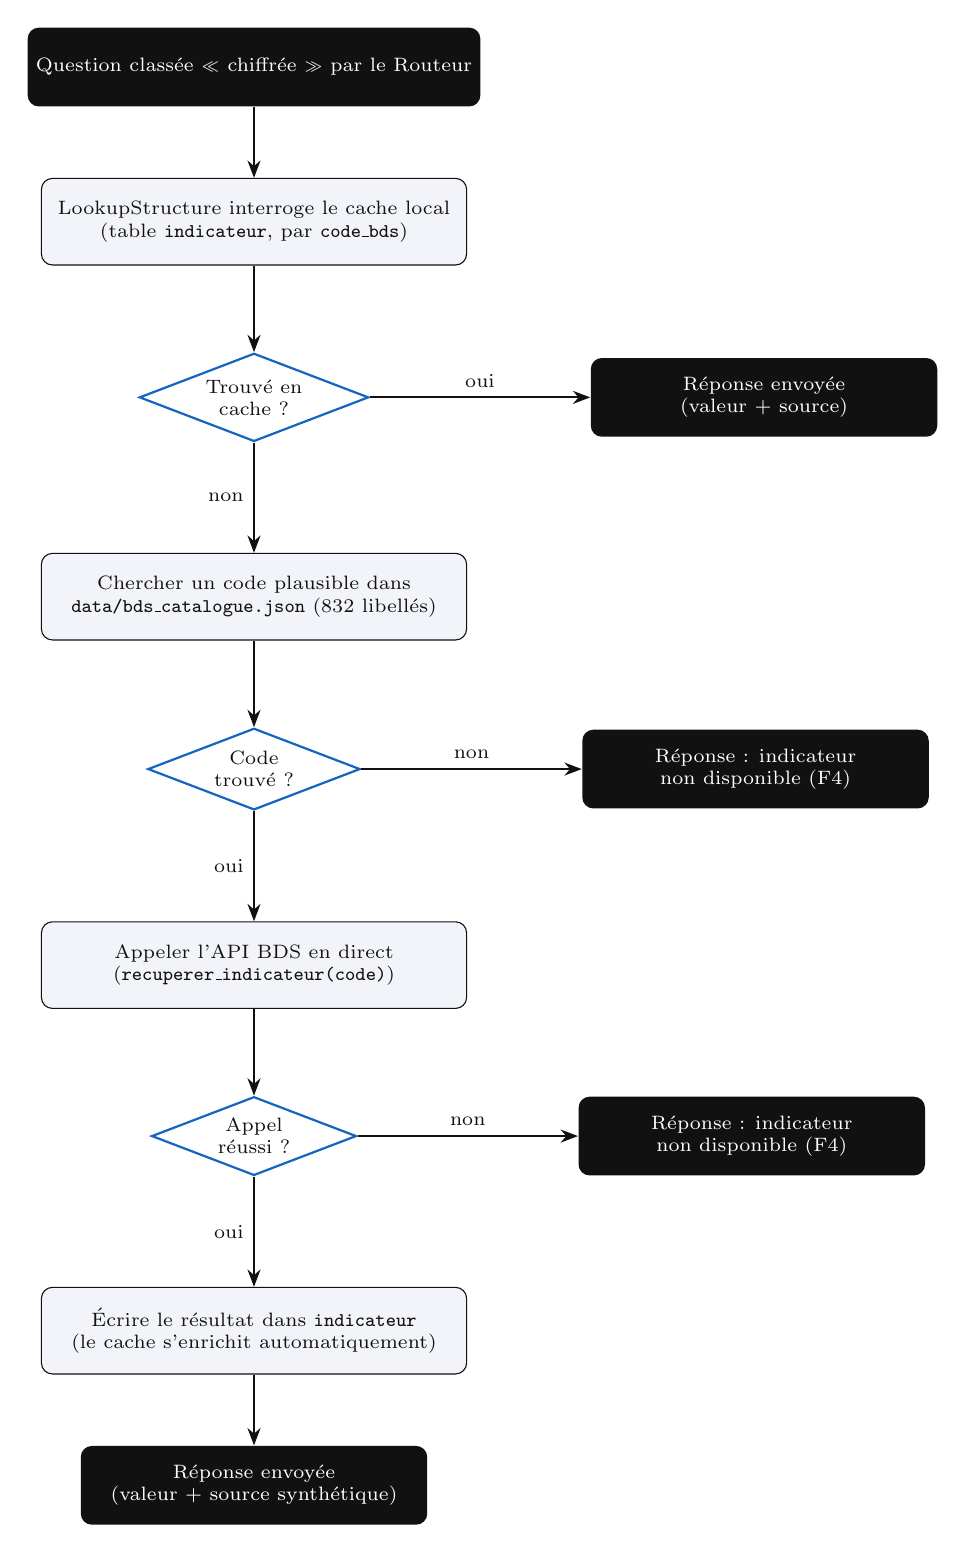
\begin{tikzpicture}[node distance=0.9cm and 1.6cm]

\node (start) [startend] {Question class\'ee \guillemotleft~chiffr\'ee~\guillemotright\ par le Routeur};
\node (p1) [process, below=of start] {LookupStructure interroge le cache local\\(table \texttt{indicateur}, par \texttt{code\_bds})};
\node (d1) [decision, below=of p1, yshift=-0.2cm] {Trouv\'e en\\cache ?};
\node (e1) [startend, right=of d1, xshift=1.2cm] {R\'eponse envoy\'ee\\(valeur + source)};

\node (p2) [process, below=of d1, yshift=-0.5cm] {Chercher un code plausible dans\\\texttt{data/bds\_catalogue.json} (832 libell\'es)};
\node (d2) [decision, below=of p2, yshift=-0.2cm] {Code\\trouv\'e ?};
\node (e2) [startend, right=of d2, xshift=1.2cm] {R\'eponse~: indicateur\\non disponible (F4)};

\node (p3) [process, below=of d2, yshift=-0.5cm] {Appeler l'API BDS en direct\\(\texttt{recuperer\_indicateur(code)})};
\node (d3) [decision, below=of p3, yshift=-0.2cm] {Appel\\r\'eussi ?};
\node (e3) [startend, right=of d3, xshift=1.2cm] {R\'eponse~: indicateur\\non disponible (F4)};

\node (p4) [process, below=of d3, yshift=-0.5cm] {\'Ecrire le r\'esultat dans \texttt{indicateur}\\(le cache s'enrichit automatiquement)};
\node (e4) [startend, below=of p4] {R\'eponse envoy\'ee\\(valeur + source synth\'etique)};

\draw[flow] (start) -- (p1);
\draw[flow] (p1) -- (d1);
\draw[flow] (d1) -- node[above, font=\scriptsize\color{gold}]{oui} (e1);
\draw[flow] (d1) -- node[left, font=\scriptsize\color{gold}]{non} (p2);
\draw[flow] (p2) -- (d2);
\draw[flow] (d2) -- node[above, font=\scriptsize\color{gold}]{non} (e2);
\draw[flow] (d2) -- node[left, font=\scriptsize\color{gold}]{oui} (p3);
\draw[flow] (p3) -- (d3);
\draw[flow] (d3) -- node[above, font=\scriptsize\color{gold}]{non} (e3);
\draw[flow] (d3) -- node[left, font=\scriptsize\color{gold}]{oui} (p4);
\draw[flow] (p4) -- (e4);

\end{tikzpicture}%
}
\par\vspace{4pt}
{\small\color{greytext}\itshape Figure A -- Lookup hybride cache-aside pour une question chiffr\'ee}
\end{figure}

\subsection*{Analyse}
Le chemin le plus court (cache trouv\'e d\`es la premi\`ere \'etape) reste tr\`es rapide~: c'est le cas majoritaire attendu, gr\^ace au pr\'e-remplissage nocturne (figure B). Les deux points de sortie \guillemotleft~indicateur non disponible~\guillemotright\ mat\'erialisent directement le besoin fonctionnel F4~: le syst\`eme ne doit jamais inventer une valeur chiffr\'ee, il doit reconna\^itre explicitement les limites de sa couverture. La derni\`ere \'etape (\'ecriture dans \texttt{indicateur} apr\`es un appel r\'eussi) est ce qui rend le cache auto-expansif~: un indicateur demand\'e une fois en direct devient disponible en cache pour toutes les questions suivantes portant sur le m\^eme code.

\section{Diagramme -- pr\'e-remplissage nocturne}
En compl\'ement du chemin \guillemotleft~\`a la demande~\guillemotright\ ci-dessus, un traitement par lot maintient le cache \`a jour pour les indicateurs les plus consult\'es, sans attendre qu'un utilisateur les demande.

\begin{figure}[h!]
\centering
\resizebox{\textwidth}{!}{%
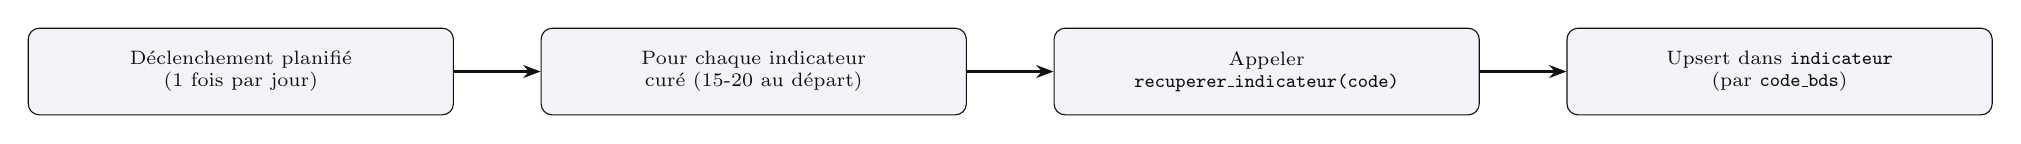
\begin{tikzpicture}[node distance=1.1cm]
\node (s1) [process] {D\'eclenchement planifi\'e\\(1 fois par jour)};
\node (s2) [process, right=of s1] {Pour chaque indicateur\\cur\'e (15-20 au d\'epart)};
\node (s3) [process, right=of s2] {Appeler\\\texttt{recuperer\_indicateur(code)}};
\node (s4) [process, right=of s3] {Upsert dans \texttt{indicateur}\\(par \texttt{code\_bds})};

\draw[flow] (s1) -- (s2);
\draw[flow] (s2) -- (s3);
\draw[flow] (s3) -- (s4);
\end{tikzpicture}%
}
\par\vspace{4pt}
{\small\color{greytext}\itshape Figure B -- Pr\'e-remplissage nocturne des indicateurs cur\'es}
\end{figure}

\subsection*{Analyse}
Cette t\^ache planifi\'ee est ind\'ependante du chemin utilisateur~: elle ne bloque jamais une r\'eponse, elle pr\'epare le terrain. L'\guillemotleft~upsert~\guillemotright\ (mise \`a jour si le \texttt{code\_bds} existe d\'ej\`a, insertion sinon) garantit que les valeurs restent align\'ees sur les derni\`eres publications de la BDS sans dupliquer de lignes \`a chaque ex\'ecution.

\section{Impact sur les modules existants}
\begin{longtable}{@{}p{3.9cm}p{12.5cm}@{}}
\rowcolor{navy}
\tblhead{Module} & \tblhead{Impact} \\
\midrule
\endhead
\texttt{LookupStructure} & Passe d'une simple requ\^ete SQL \`a la cascade d\'ecrite en figure A. Doit d\'esormais savoir interroger \texttt{data/bds\_catalogue.json} et appeler \texttt{src/bds\_client.py} en repli. \\
\texttt{ConstructeurIndicateurs} & Reste responsable des indicateurs extraits de PDF/XLSX (\texttt{code\_bds IS NULL}), mais n'est plus la seule voie d'alimentation de la table \texttt{indicateur}~: le pr\'e-remplissage nocturne et le repli en direct l'alimentent aussi, via \texttt{code\_bds}. \\
\texttt{Scraper} / \texttt{Extracteur} & Inchang\'es. Toujours n\'ecessaires pour le texte narratif et les publications hors catalogue BDS (ADR 0003). \\
\texttt{Interface} / \texttt{Generateur} & Inchang\'es dans leur r\^ole~: mettre en forme et citer la source. La source cit\'ee peut d\'esormais \^etre soit un vrai document collect\'e, soit une fiche synth\'etique \texttt{api}. \\
\end{longtable}

\section{Synth\`ese}
Ce compl\'ement referme les deux points laiss\'es ouverts par l'ADR 0004~: la tra\c{c}abilit\'e (r\'esolue par le document synth\'etique de type \texttt{api}) et la fra\^icheur des donn\'ees (r\'esolue par la strat\'egie cache-aside hybride, figures A et B). Le sch\'ema relationnel et le diagramme de classes originaux restent valides sans modification structurelle~: seuls deux colonnes et le comportement de \texttt{LookupStructure} \'evoluent. La prochaine \'etape est la validation en conditions r\'eelles de \texttt{src/bds\_client.py}, premi\`ere t\^ache du backlog Sprint 2.

\end{document}
